%\thispagestyle{empty}
\section{CONCLUSÃO}
Para conluir irei mostrar os resultados dos teste de cada algoritmo com as duas bases de dados e faz no final fazer um comparativo entre o desempenho dos algoritmos.

O algoritmo de regressão linear com a base1\footnote[4]{base de dados de 2014 a 2018 com 9.840 jogo} teve um taxa de acerto de 65\%, veja o grafico de relação entre os dados reais e os previstos. Após aplicar \textit{Cros Validation} o essa taxa teve um aumento de 2\%.
\begin{figure}[htbp]
	\begin{center}
		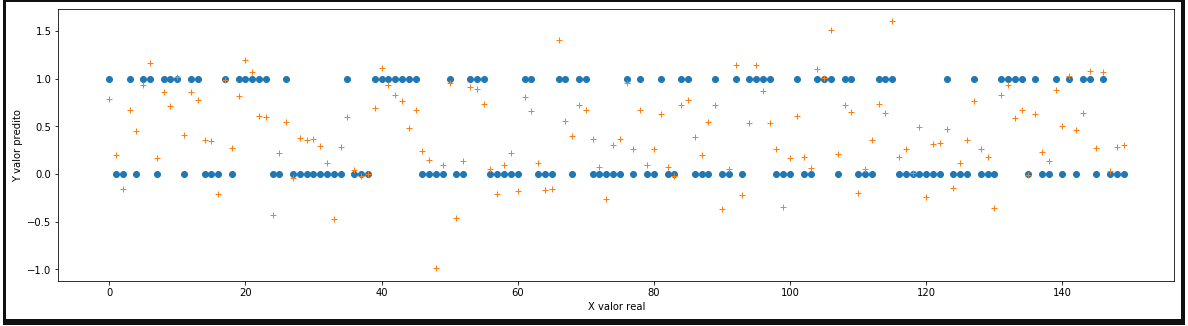
\includegraphics[width=0.7\linewidth]{imagens/regressailinear.png}\\
	\end{center}
	\caption[relação entre os dados reais e os previstos]{relação entre os dados reais e os previstos}
	\label{fig:logo}
	%%\legend{Fonte: Próprio Autor}
\end{figure}

O algoritmo de regressão linear com a base2\footnote[5]{base de dados de 2007 a 2019 com 30.000 jogos} teve um taxa de acerto de 68\%, veja o grafico de relação entre os dados reais e os previstos. Após aplicar o \textit{Cros Validation} essa taxa teve um aumento de 3.6\%.
\begin{figure}[htbp]
	\begin{center}
		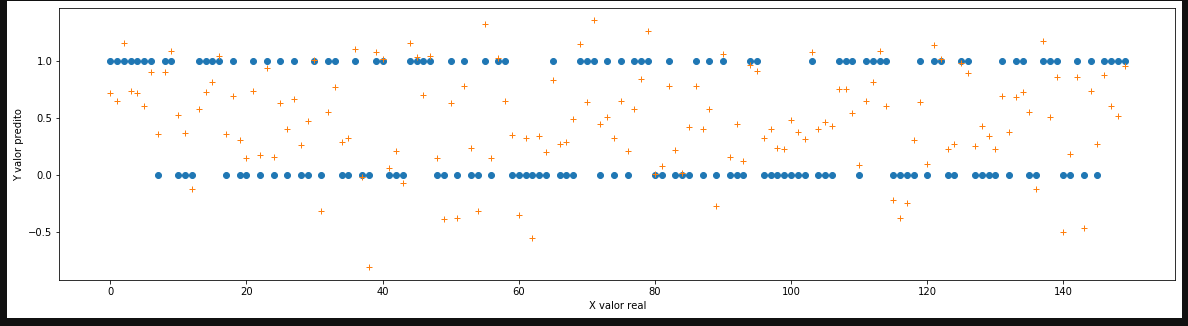
\includegraphics[width=0.7\linewidth]{imagens/regressailinearAPI.png}\\
	\end{center}
	\caption[relação entre os dados reais e os previstos]{relação entre os dados reais e os previstos}
	\label{fig:logo}
	%%\legend{Fonte: Próprio Autor}
\end{figure}

O algoritmo de arvore decisão com a base1\footnote[4]{base de dados de 2014 a 2018 com 9.840 jogo} teve um taxa de acerto de 89.7\%, veja o grafico de relação entre os dados reais e os previstos. Após aplicar o \textit{Cros Validation} essa taxa teve um aumento de 4\%.
\begin{figure}[htbp]
	\begin{center}
		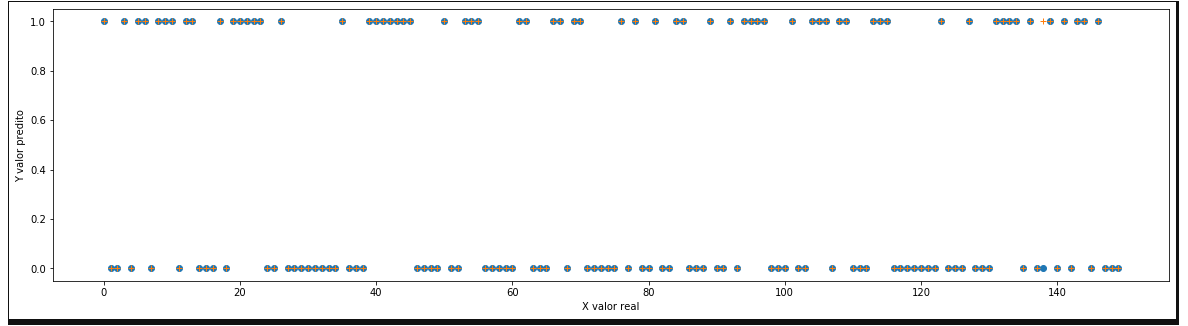
\includegraphics[width=0.7\linewidth]{imagens/arvoredecisao.png}\\
	\end{center}
	\caption[relação entre os dados reais e os previstos]{relação entre os dados reais e os previstos}
	\label{fig:logo}
	%%\legend{Fonte: Próprio Autor}
\end{figure}

O algoritmo de arvore decisão com a base2\footnote[5]{base de dados de 2007 a 2019 com 30.000 jogos} teve um taxa de acerto de 97\%, veja o grafico de relação entre os dados reais e os previstos. Após aplicar o \textit{Cros Validation} essa taxa teve um  aumento de 3\%.
\begin{figure}[htbp]
	\begin{center}
		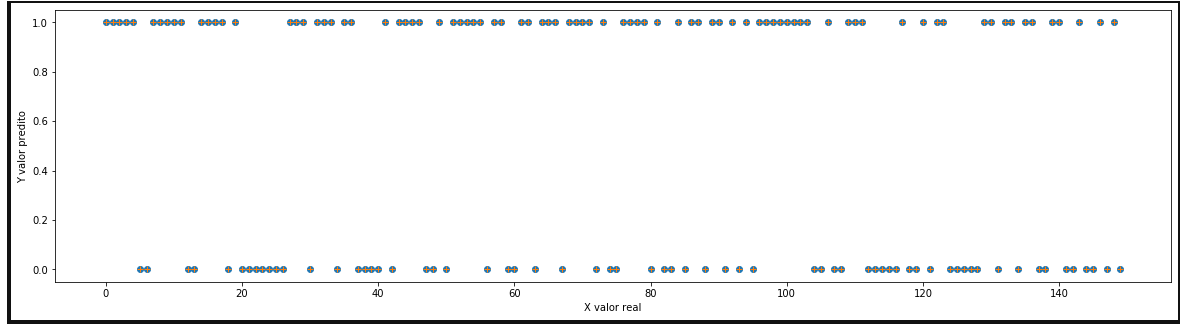
\includegraphics[width=0.7\linewidth]{imagens/arvoredecisaoAPI.png}\\
	\end{center}
	\caption[relação entre os dados reais e os previstos]{relação entre os dados reais e os previstos}
	\label{fig:logo}
	%%\legend{Fonte: Próprio Autor}
\end{figure}

O algoritmo de k-NN\footnote[3]{k-nearest neighbors} com a base1 teve um taxa de acerto de 85\%, veja o grafico de relação entre os dados reais e os previstos. Após aplicar o \textit{Cros Validation} essa taxa teve um aumento de 2.8\%.
\begin{figure}[htbp]
	\begin{center}
		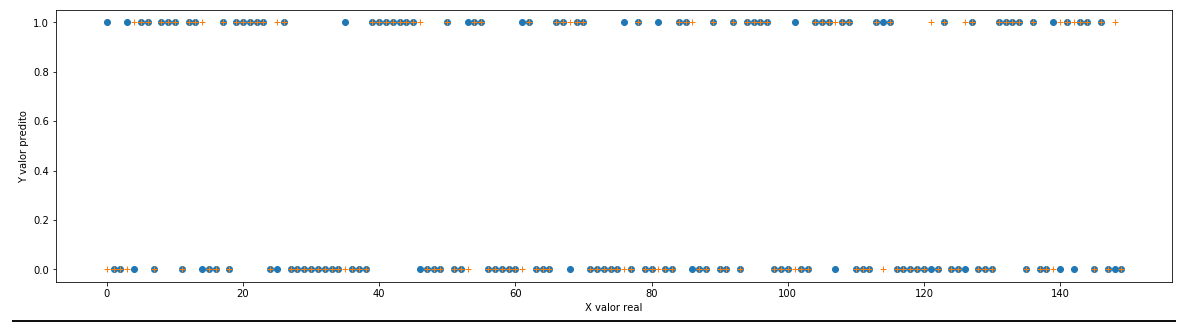
\includegraphics[width=0.7\linewidth]{imagens/knn.png}\\
	\end{center}
	\caption[relação entre os dados reais e os previstos]{relação entre os dados reais e os previstos}
	\label{fig:logo}
	%%\legend{Fonte: Próprio Autor}
\end{figure}

O algoritmo de k-NN\footnote[3]{k-nearest neighbors} com a base2\footnote[5]{base de dados de 2007 a 2019 com 30.000 jogos} teve um taxa de acerto de 87\%, veja o grafico de relação entre os dados reais e os previstos.Após aplicar o \textit{Cros Validation} essa taxa teve um aumento de 3.3\%.
\begin{figure}[htbp]
	\begin{center}
		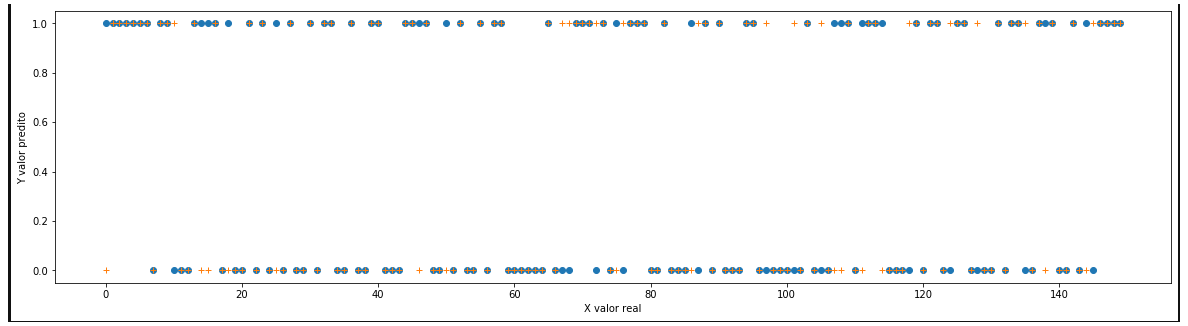
\includegraphics[width=0.7\linewidth]{imagens/knnAPI.png}\\
	\end{center}
	\caption[relação entre os dados reais e os previstos]{relação entre os dados reais e os previstos}
	\label{fig:logo}
	%%\legend{Fonte: Próprio Autor}
\end{figure}

O algoritmo de floresta aleatória com a base2 inicialmente foi testado com 10 arvores chegando a um resultado de 94\% na taxa de acerto.
\begin{figure}[htbp]
	\begin{center}
		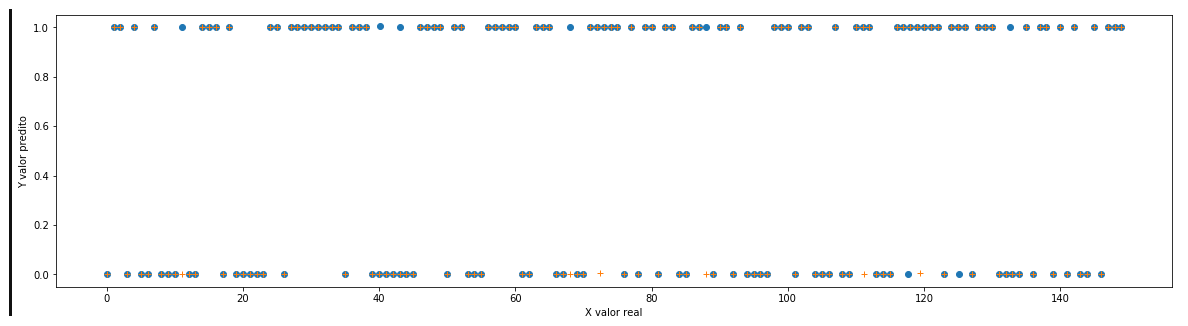
\includegraphics[width=0.7\linewidth]{imagens/florestaaleatoria.png}\\
	\end{center}
	\caption[relação entre os dados reais e os previstos com 10 arvores]{relação entre os dados reais e os previstos com 10 arvores}
	\label{fig:logo}
	%%\legend{Fonte: Próprio Autor}
\end{figure}

O algoritmo de floresta aleatória com a base2 o teste com 53 arvores o teste conseguiu atingir uma faixa de os 99\% e 100\% de precisão. Para sempre ter um taxa contante de 100\% de acerto são necessária mais de 100 arvores.
\begin{figure}[htbp]
\begin{center}
	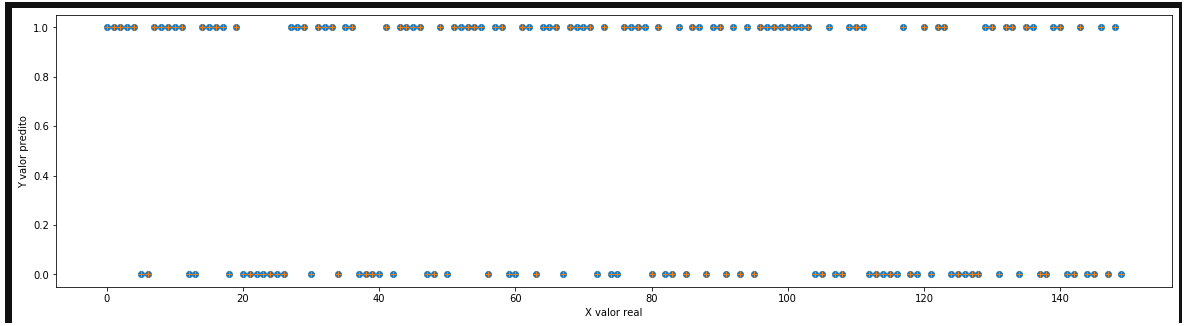
\includegraphics[width=0.7\linewidth]{imagens/florestaaleatoriaAPI.png}\\
\end{center}
\caption[relação entre os dados reais e os previstos com 53 arvores]{relação entre os dados reais e os previstos com 53 arvores}
\label{fig:logo}
%%\legend{Fonte: Próprio Autor}
\end{figure}
\newpage
O algoritmo de regressão logística tanto com a base1\footnote[4]{base de dados de 2014 a 2018 com 9.840 jogo} é com a  base2\footnote[5]{base de dados de 2007 a 2019 com 30.000 jogos} teve um taxa de acerto de 100\%, veja o grafico de relação entre os dados reais e os previstos.
\begin{figure}[htbp]
	\begin{center}
		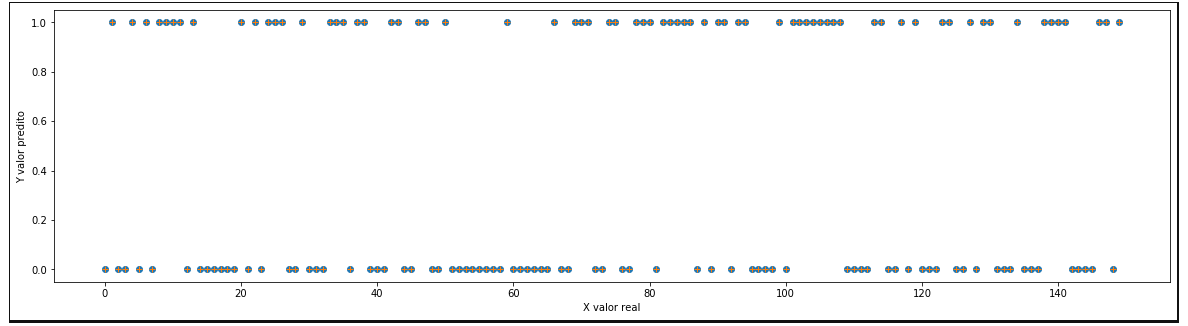
\includegraphics[width=0.7\linewidth]{imagens/regressaologistocaAPI.png}\\
	\end{center}
	\caption[relação entre os dados reais e os previstos]{relação entre os dados reais e os previstos}
	\label{fig:logo}
	%%\legend{Fonte: Próprio Autor}
\end{figure}

O algoritmo de máquinas de vetores de suporte com a base1 teve um taxa de acerto de 80\%, veja o grafico de relação entre os dados reais e os previstos.
\begin{figure}[htbp]
	\begin{center}
		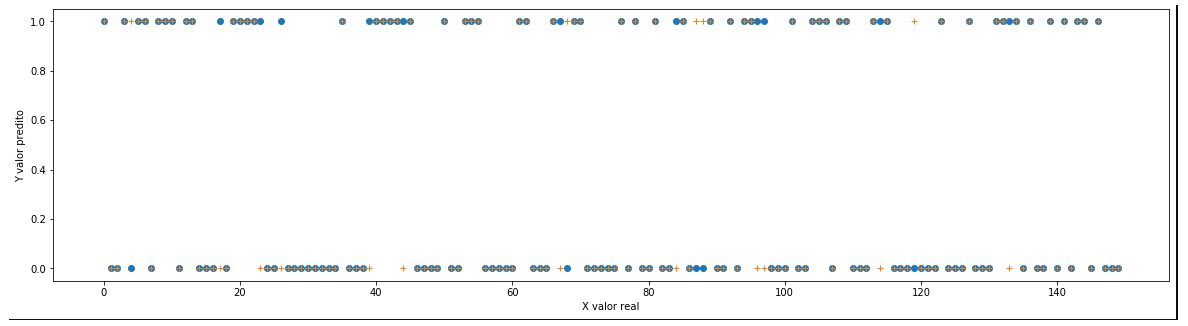
\includegraphics[width=0.7\linewidth]{imagens/SVM.png}\\
	\end{center}
	\caption[relação entre os dados reais e os previstos]{relação entre os dados reais e os previstos}
	\label{fig:logo}
	%%\legend{Fonte: Próprio Autor}
\end{figure}

O algoritmo de máquinas de vetores de suporte com a base1 teve um taxa de acerto de 87\%, veja o grafico de relação entre os dados reais e os previstos.
\begin{figure}[htbp]
	\begin{center}
		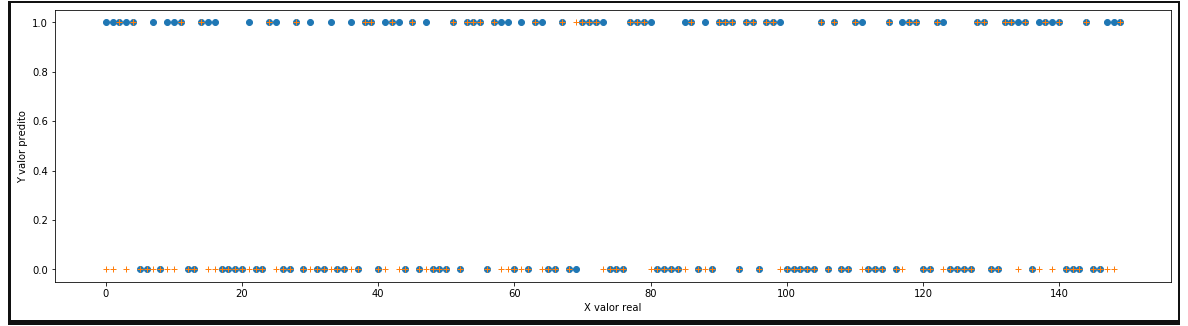
\includegraphics[width=0.7\linewidth]{imagens/SVMAPI.png}\\
	\end{center}
	\caption[relação entre os dados reais e os previstos]{relação entre os dados reais e os previstos}
	\label{fig:logo}
	%%\legend{Fonte: Próprio Autor}
\end{figure}
\newpage

O algoritmo de regressão linear que teve o pior despenho no teste, devido a construção dele trabalhar melhor com dados lineares. O que dado que foi utilizado consistia em prever derrota ou vitoria ou seja, o valor da predição era de forma binaria. Assim a técnicas de regressão linear procuram a relação entre duas variáveis por meio de uma equação de uma linha reta.

O algoritmos arvore de decisão, como funciona na forma de um fluxograma em pra suas tomadas de decisão vai depender da quantidade e qualidade dos dados com a qual essa arvore foi treinada. Como pode ser visto nos resultado a taxa de acertos com a utilização da base1\footnote[4]{base de dados de 2014 a 2018 com 9.840 jogo}, quando testado um a base2\footnote[5]{base de dados de 2007 a 2019 com 30.000 jogos} que possui mais que o dobre de dados a taxa teve um grande aumento.

o algoritmo k-NN\footnote[3]{k-nearest neighbors} trabalho com os vizinhos mais deve ser considerado como um método
no qual baseia-se por instâncias, isto é, ele vai determinar a classe de um objeto
desconhecido através da classe de outras instâncias.

As floresta aleatória e um conjunto de arvores de decisão trabalhando em conjunto, com um maior numero de arvore a taxa de predição também aumenta. Nos teste realizados com 10 arvores tinha uma aula porcentagem de acertos quando chegando acima de 53 arvore a taxa varia de 99\% a 100\%, mas quanto o maior numero de arvores o tempo do teste vai aumentando significativamente. Para ter uma taxa de constante de 100\% seria necessario mas 100 arvores isso exige um grande tempo.

A regressão logística foi o algoritmo com a maior taxa de acertos, pois ele trabalho com so fatores binário de predição,sendo assim o opostos da regressão linear. Como os teste foram feitos para prever a derrota e a vitoria.Assim a regressão logística calcula uma razão de probabilidade da variável alvo, que posteriormente é convertida em uma variável de base logarítmica, permitindo assim a classificação com base na aproximação de um dos valores. 

A máquinas de vetores trabalha definindo um limite linear logo para realizar a
classificação ele separa os dados é os analisa para reconhecer padrões, assim que a uma entrada de um conjunto de dados e adicionada ele vai realizar a analise e dividir em duas classes, na qual as duas possíveis classes faz parte do classificador linear binário não probabilístico.





